\documentclass[sigconf,anonymous]{acmart}

\setcopyright{none}
\settopmatter{printacmref=true,printfolios=true}
\renewcommand\footnotetextcopyrightpermission[1]{}
\acmConference[DAI 2026]{The Eighth International Conference on Distributed Artificial Intelligence}{November 29--December 2, 2026}{Hong Kong, China}
\acmBooktitle{The Eighth International Conference on Distributed Artificial Intelligence (DAI 2026)}
\acmYear{2026}
\acmDOI{}
\acmISBN{}

\usepackage{booktabs}
\usepackage{graphicx}
\usepackage{xcolor}
\usepackage{placeins}
\graphicspath{{figures/}}

\newcommand{\heard}{\textsc{Heard}}
\newcommand{\said}{\textsc{Said}}
\newcommand{\held}{\textsc{Held}}
\newcommand{\prov}{\textsc{Prov}}
\newcommand{\apm}{\textsc{Apm}}
\newcommand{\ga}{\textsc{Ga}}
\newcommand{\cellci}[2]{\shortstack[c]{#1\\[-1.5pt]\textcolor{gray}{[#2]}}}

\title[Said in Public, Lost in Recall]{Said in Public, Lost in Recall: Why LLM Agent Societies Need Provenance-Aware State Updates}

\author{Anonymous Author(s)}
\affiliation{%
  \institution{Anonymous Institution}
  \country{}
}

\begin{document}

\begin{abstract}
When a fact changes in an LLM agent society, the transcript can look corrected before the society
has actually updated.  We expose this failure in a 25-agent telephone-style task that follows an
event update from received evidence (\heard), through public utterances (\said), to private
retrieval (\held).  Keeping an authoritative source active raises the pooled current-mention share
among value-bearing utterances from 62.9\% to 81.8\% ($+18.9$ points, descriptive), yet current
private answers move only from 12.0\% to 15.2\% ($+3.2$ points, 95\% CI $-5.6$ to 12.0).
Authority therefore changes what is publicly visible without producing a supported gain in what
the population can retrieve.

Where does the update disappear?  We freeze every listener's received evidence and replay the same
ordered streams through alternative memories.  Provenance-aware integration raises current answers
from 32.0\% to 60.5\% over a Generative-Agents-style pipeline ($+28.5$ points, 95\% CI
21.5--35.5), and retains a $+26.0$-point gain on independently generated streams supplied with
controlled-task versions.  In a stricter matched ablation, changing only conflict selection from
mention frequency to maximum version adds 9.0 points (95\% CI 4.4--13.6).  These interventions
identify listener-side integration as one causal locus and support a simple design principle:
mutable facts should be treated as ordered state changes, not popularity contests among repeated
claims.

The repair, however, reveals a second bottleneck.  Default dialogue preserves no parseable
source/version marker in 720 utterances, and unauthenticated versions can be forged.  Reliable
agent societies therefore require more than a better memory module: they need a provenance-aware
state-update protocol that preserves, resolves, and authenticates updates between communication
and memory---alongside evaluation that tests what agents can retrieve rather than only what their
transcripts display.
\end{abstract}

\begin{CCSXML}
<ccs2012>
 <concept>
  <concept_id>10010147.10010178.10010219</concept_id>
  <concept_desc>Computing methodologies~Multi-agent systems</concept_desc>
  <concept_significance>500</concept_significance>
 </concept>
 <concept>
  <concept_id>10010147.10010257.10010258.10010259</concept_id>
  <concept_desc>Computing methodologies~Natural language generation</concept_desc>
  <concept_significance>300</concept_significance>
 </concept>
</ccs2012>
\end{CCSXML}

\ccsdesc[500]{Computing methodologies~Multi-agent systems}
\ccsdesc[300]{Computing methodologies~Natural language generation}
\keywords{LLM agents, multi-agent systems, social simulation, memory, provenance, misinformation}

\begin{teaserfigure}
  \centering
  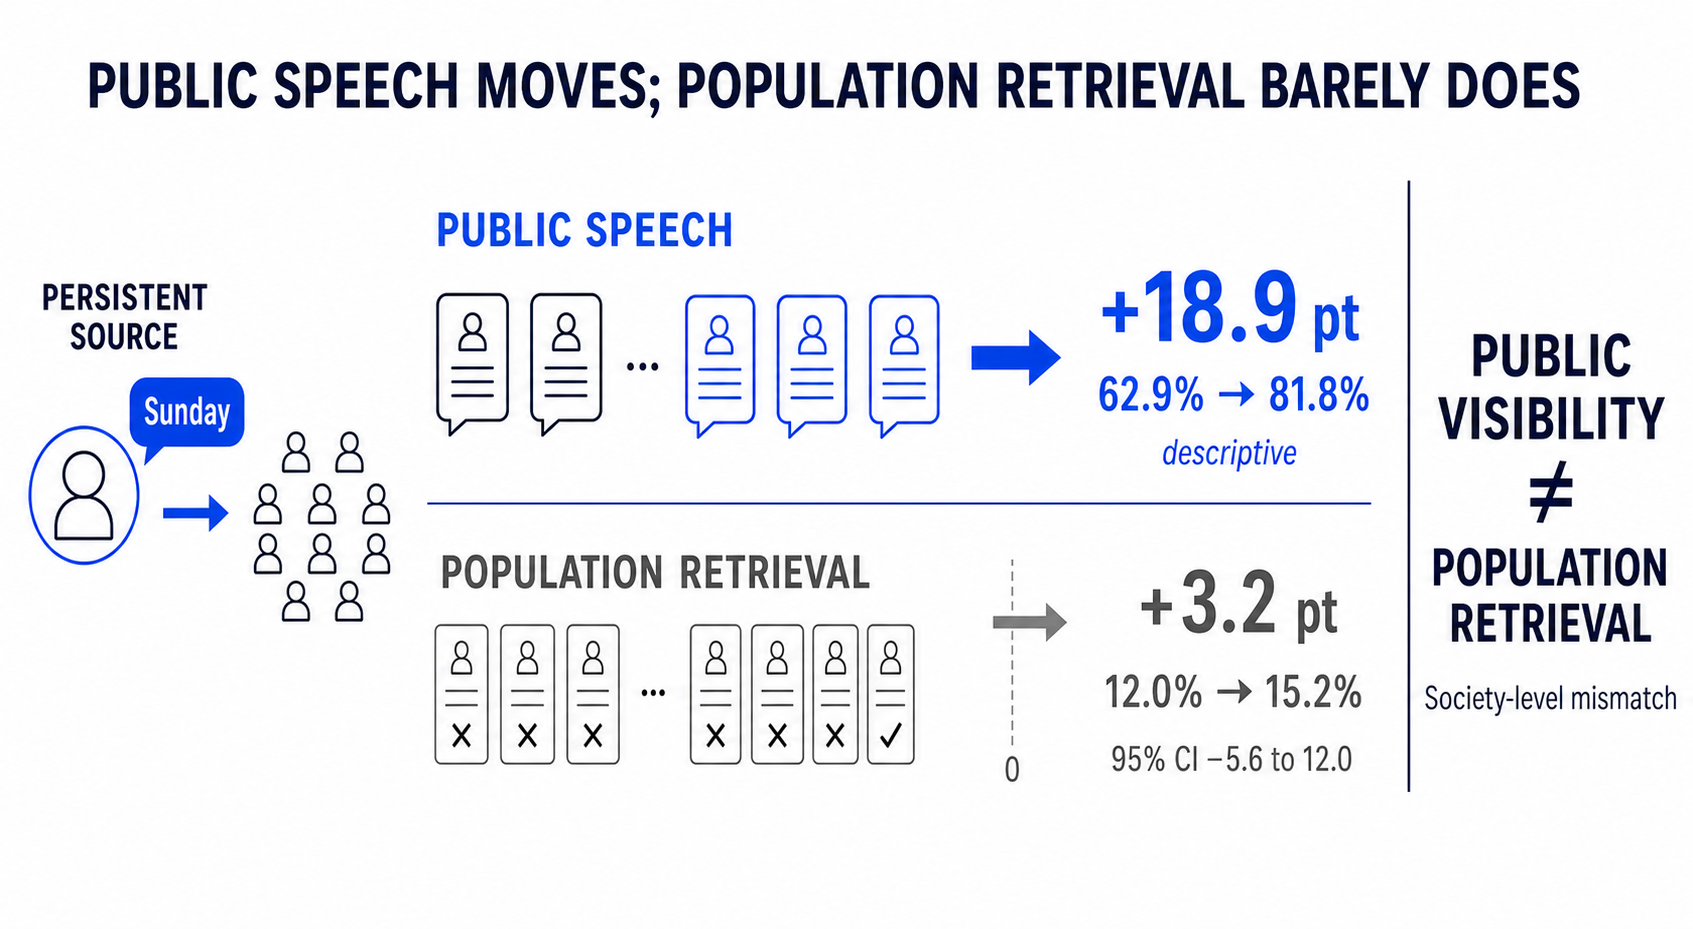
\includegraphics[width=0.88\textwidth,trim=0 0 0 125,clip]{figures/story_redesign/fig1_public_private_v1.png}
  \caption{Speech is not retrieval.  A persistent source changes the
  pooled current-mention share by $+18.9$ points but private current answers by only $+3.2$ points
  (95\% CI $-5.6$ to 12.0), revealing a society-level mismatch.}
  \Description{A persistent source introduces Sunday into an agent society.  Public speech moves
  by 18.9 points, whereas population-wide private retrieval moves by 3.2 points with a confidence
  interval spanning zero.  The figure summarizes a society-level mismatch between public
  visibility and population retrieval.}
  \label{fig:core}
\end{teaserfigure}

\maketitle

\section{Introduction}

LLM-based agent societies increasingly coordinate through conversation: they simulate
communities, negotiate plans, deliberate, and divide work
\cite{park2023generative,li2023camel,wu2023autogen,zhou2024sotopia}.  Their success is therefore
often read from the conversation itself.  If the corrected fact appears repeatedly in a public
transcript, the society seems corrected.  But the transcript is a public record, not the
retrievable state of the agents that must later act.  A fact may win the conversation without
updating the society.

This distinction becomes critical when facts change.  Standard conversational memories rank
observations by recurrence, relevance, or salience.  Those signals are useful for recalling a
topic, but a mutable fact is not a majority vote: ten repetitions of an obsolete value should not
override one authenticated update.  Reliable coordination therefore requires more than
transmission.  It requires a rule that turns received claims into an ordered, retrievable state.
Existing transcript-level evaluations blur these operations and cannot show where an update is
lost.

We make the loss observable with a minimal changing-fact probe.  A society of 25 agents initially
knows an obsolete event time and location; one source then receives the current value, and agents
propagate it through pairwise conversation.  We follow the update across three operational stages:
\heard{}, evidence received by an agent; \said{}, claims present in public utterances; and
\held{}, the answer returned in a private post-transmission interview.  ``Held'' denotes an
elicited behavior, not a literal mental state.  The separation reveals the paper's central
observation: an authoritative source can make the update more visible in public speech without a
supported increase in population-wide private retrieval.

We then ask a narrower question than whether a model can state the truth: given exactly the same
received evidence, which memory operation determines what a listener later returns?  Matched-event
replays freeze each agent's realized stream before comparing complete listener-side memories.
A stricter ablation holds representation, candidates, retrieval, context, and interview fixed
while changing only conflict selection from mention frequency to maximum version.  Together these
interventions locate one failure inside listener integration and test provenance-aware updating as
a repair.  Follow-up channel and attack tests establish the repair's boundary: provenance must
survive relay and be authenticated before a version can safely govern state.

This paper makes three contributions:
\begin{enumerate}
  \item an empirical finding: public uptake and population retrieval can diverge, which makes
  transcript-only success an incomplete measure of social coordination;
  \item a causal diagnosis: fixed-stream interventions locate part of the failure in
  listener-side integration and isolate the benefit of version priority over repetition; and
  \item a protocol-level design principle: mutable facts require a communication--memory
  interface that preserves and authenticates provenance before applying ordered state updates.
\end{enumerate}

\section{Related Work}

\paragraph{LLM agent societies and communication}
Generative Agents established memory, reflection, and retrieval as a basis for believable
long-horizon social behavior \cite{park2023generative}; CAMEL, AutoGen, and SOTOPIA developed
communicative multi-agent interaction and social evaluation
\cite{li2023camel,wu2023autogen,zhou2024sotopia,chen2023agentverse}.  Population-scale simulation
and role-specialized frameworks broaden this setting
\cite{park2024thousand,hong2024metagpt,qian2024chatdev,gao2024agentscope}, while theory-of-mind
reasoning, communication-graph design, and learned message representations target coordination
more directly \cite{li2023theorymind,zhang2025gdesigner,ramesh2025activations}.  Debate-oriented
systems study whether interaction improves task accuracy
\cite{du2023improving,michael2023debate,liang2024encouraging,khan2024debating}, although protocol
comparisons show that gains are sensitive to design choices \cite{smit2024mad}.  Failure
taxonomies and adversarial studies further expose specification, verification, and compounding
error problems \cite{cemri2025mast,gu2024agentsmith,amayuelas2024multiagent,xie2026spark,
jia2026masfire}.  We study decentralized propagation of a changed fact rather than a centralized
final decision or a generic coordination failure.

\paragraph{Public expression and private agent state}
Several adjacent studies show why transcripts alone are insufficient.  Persona simulations compare
pre- and post-discussion private responses with chat transcripts and find conformity and
instability \cite{baltaji2024conformity,weng2025conformity}.  Think-Before-Speak explicitly
separates structured internal evaluation from public expression in social simulation
\cite{yang2026think}.  Embodied-agent work measures alignment between private world models and
finds that dialogue can reduce action conflict while degrading task success
\cite{dongre2026worldmodels}.  Our distinction is operational and fact-specific: \heard{} records
received events, \said{} measures claims in public utterances, and \held{} probes the answer
retrieved after transmission.  We then intervene on the listener's memory rule rather than only
describing a public/private gap.

\paragraph{Misinformation, conformity, and factuality}
Human misinformation research distinguishes exposure and diffusion from durable correction
\cite{lazer2018science,vosoughi2018spread,lewandowsky2012misinformation,thorson2016belief}.
Factuality benchmarks and detectors likewise treat semantic truth as distinct from surface
plausibility
\cite{lin2022truthfulqa,manakul2023selfcheckgpt,farquhar2024detecting,li2023halueval,
niu2024ragtruth}.  Rumor cascades, LLM-mediated misinformation, and audience-tuned language show
that transmission can transform both content and expression
\cite{friggeri2014rumor,maurya2025simulating,beukeboom2019stereotypes,ye2021audience}, whereas
epidemic and randomized rumor-spreading algorithms characterize reach and latency under explicit
message semantics \cite{demers1987epidemic,karp2000rumor}.  Our
current/stale/unknown verdict is analogous to three-way fact verification
\cite{thorne2018fever}, but is applied to post-communication agent answers.  Attacks on
multi-agent collaboration and concurrent work on error cascades examine how false inputs spread
and how centralized governance may suppress them
\cite{amayuelas2024multiagent,xie2026spark}.  Our complementary setting starts from a valid
correction to a formerly true fact, probes each listener privately, and evaluates a local memory
interface.

\paragraph{Agent memory and belief revision}
Long-term agent memories improve storage, retrieval, and organization
\cite{zhong2024memorybank,packer2024memgpt,xu2025amem,chhikara2025mem0}; probabilistic belief
memory retains competing uncertain conclusions under partial observability
\cite{liao2026belief}.  Reflection and acting systems use textual memory to improve sequential
decisions \cite{shinn2023reflexion,yao2023react,wang2023voyager}, while factual editing changes
parameters rather than an agent's external memory interface \cite{meng2022rome,meng2023memit}.
We compare controlled motif adaptations under a common harness, not the official systems end to
end.  Provenance itself is not new: truth-maintenance and belief revision
formalize how new information supersedes prior commitments
\cite{doyle1979truth,alchourron1985logic}, while data provenance records origin and derivation
\cite{buneman2001provenance,moreau2013provdm} and opinion dynamics studies source-weighted
updating \cite{degroot1974reaching}.  Our contribution is an empirical bridge between these lines:
under frozen social evidence, supplied versions affect listener integration, but the benefit is
bounded by whether the communication channel preserves and authenticates them.

\section{Following an Update from Speech to State}

\subsection{A changing-fact telephone game}

The central story requires separating three questions that a transcript normally conflates:
did an agent receive the update, did the update appear in public speech, and could the agent
retrieve it afterward?  We operationalize those questions in the harness behind
Figure~\ref{fig:overview}.  A society contains $N=25$ agents connected by a
contact graph.  The agents initially discuss a stale event value $v_0$ (Saturday at the front
porch).  At round 1, the environment gives one designated source the current value $v_1$ (Sunday
at the community center).  During each round, scheduled pairs exchange natural-language
utterances.  Each agent observes both sides of its encounters, consolidates those observations
into memory, and retrieves memory to condition later speech.  After the final round, a separate
interview asks each agent when and where the event is now held.

\begin{figure*}[t]
  \centering
  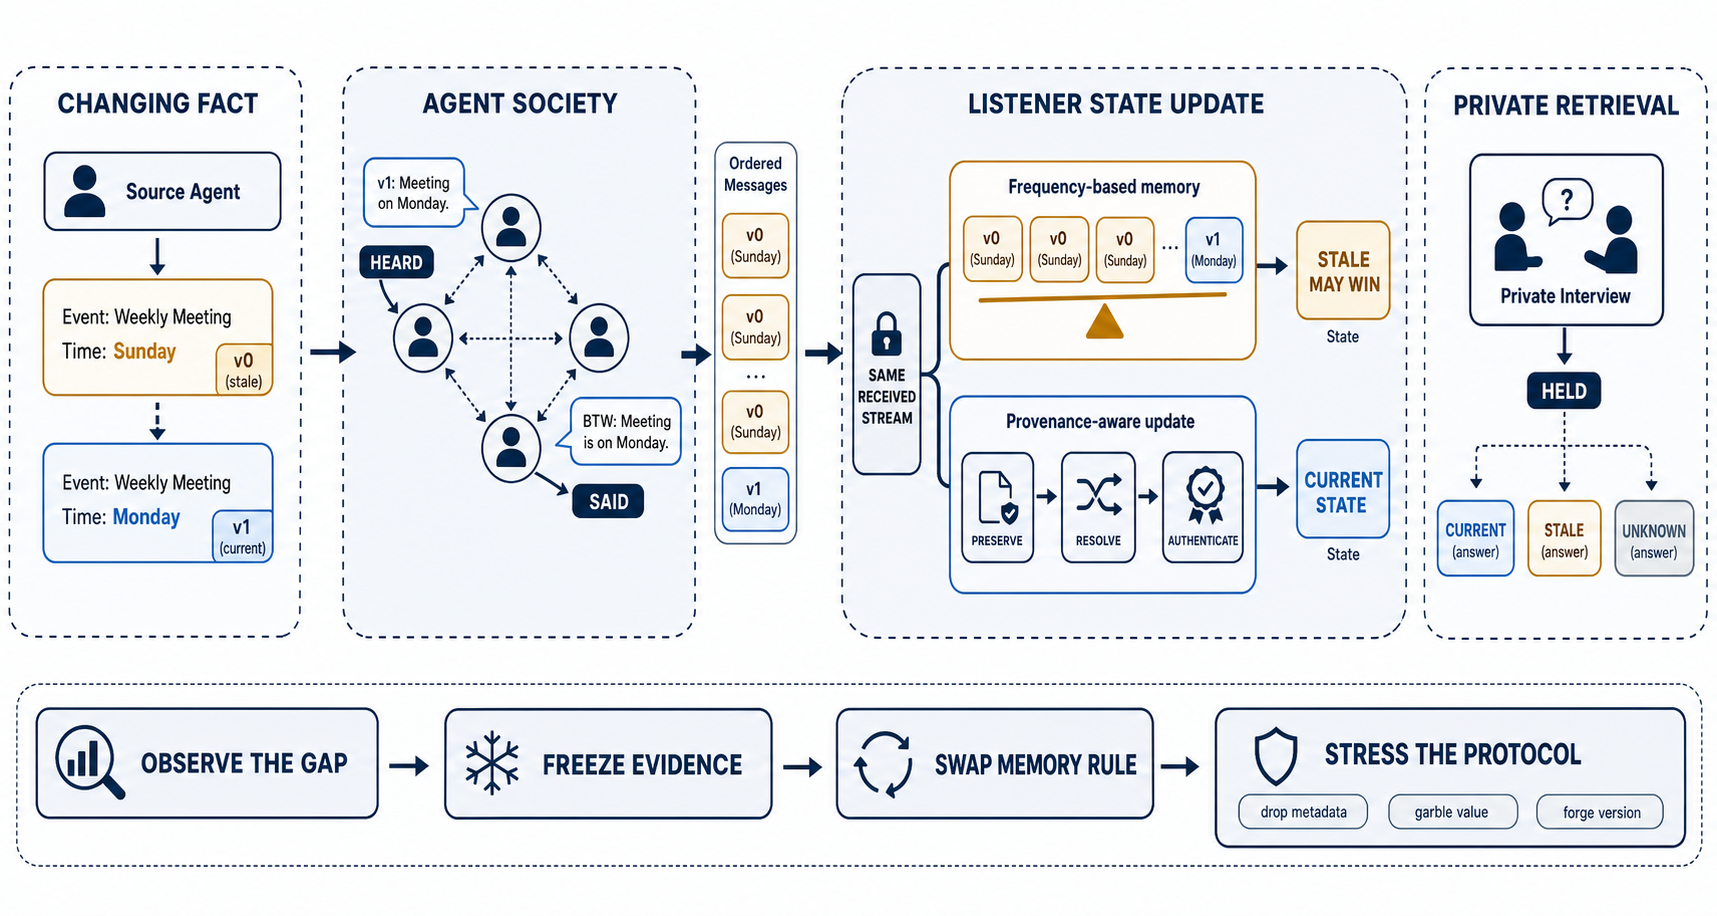
\includegraphics[width=\textwidth]{story_redesign/fig2_method_overview_image2_v1.png}
  \caption{From speech to state.  We observe \heard{}, \said{}, and \held{}, then freeze each
  received stream and replace only the listener's update rule.  Channel and attack tests stress
  preservation, resolution, and authentication.}
  \Description{A changing fact propagates through an agent society as heard evidence and public
  speech.  The same received stream enters either frequency-based memory, where repeated stale
  mentions may win, or a provenance-aware update that preserves, resolves, and authenticates the
  current state.  A private interview measures held answers.  A lower strip summarizes the
  observational gap, fixed-evidence replay, memory-rule intervention, and protocol stress tests.}
  \label{fig:overview}
\end{figure*}

Each scenario registers surface markers for its current and stale event values.  The deterministic
interview scorer assigns \emph{current} when an answer contains at least one current marker and no
stale marker, \emph{stale} whenever a stale marker appears (including a mixed answer), and
\emph{unknown} otherwise.  The three-way split distinguishes omission from active return of
superseded content.  \said{} measures current mentions among final-round utterances that contain
at least one registered value marker; current and stale mention flags are non-exclusive for mixed
utterances.  \held{} is the current share among all private interviews.  \heard{} denotes the
ordered evidence record delivered to a listener; reach and evidence composition are derived from
that record without assuming that receipt implies adoption.

The primary verdict is a deterministic marker classifier parameterized by the registered current
and stale values for each scenario.  We audited all 375 interview answers in the repair-drive
baseline, source, and broadcast experiment with a separate semantic LLM judge.  Agreement was
374/375 overall: 124/125 baseline answers and all 250 source and broadcast answers.
Both scorers produced the same current counts in every condition.  This validates the headline
interview metric on the core sample; it does not validate every auxiliary scenario or every
free-form claim in the transcripts.

\subsection{Formalization}

Let $q$ index an experimental condition, $r\in\{1,\ldots,K_q\}$ a schedule seed, and
$i\in\{1,\ldots,N\}$ an agent.  Let $U_{qrT}$ be the final-round public utterances and
$h_{qri}\in\{c,s,\varnothing\}$ the verdict on agent $i$'s private interview answer.  For any text
$x$, $C(x)$ and $S(x)$ indicate a registered current or stale marker, and
$V(x)=C(x)\lor S(x)$ indicates a value-bearing text.  The two society-level readouts are
\[
 \begin{aligned}
 \mathrm{Said}_{qr}
   &=\frac{\sum_{u\in U_{qrT}}\mathbb{1}[C(u)]}
           {\sum_{u\in U_{qrT}}\mathbb{1}[V(u)]},\\
 \mathrm{Held}_{qr}
   &=\frac{1}{N}\sum_{i=1}^{N}\mathbb{1}[h_{qri}=c].
 \end{aligned}
\]
The headline \said{} statistic pools its numerator and denominator across seeds and is descriptive;
\held{} is averaged within each seed, with seeds as the independent units for intervals and paired
tests.  Mixed utterances may satisfy both $C$ and $S$, but enter the \said{} denominator once;
unknown and stale interviews remain in the \held{} denominator.  The full ordered evidence record
is \heard{}; Appendix~\ref{app:exposure} defines its reach and composition summaries.

The central dissociation is a contrast between conditions, not the numerical subtraction of
\said{} and \held{}:
\[
 \begin{aligned}
 \Delta_{\mathrm{Said}}
   &=\mathrm{Said}_{\mathrm{source}}^{\mathrm{pool}}
     -\mathrm{Said}_{\mathrm{baseline}}^{\mathrm{pool}},\\
 \Delta_{\mathrm{Held}}
   &=\frac{1}{K}\sum_{r=1}^{K}
     \left(\mathrm{Held}_{\mathrm{source},r}
     -\mathrm{Held}_{\mathrm{baseline},r}\right).
 \end{aligned}
\]
Empirically, the pooled descriptive $\Delta_{\mathrm{Said}}=18.9$ percentage points, whereas
$\Delta_{\mathrm{Held}}=3.2$ points (95\% CI $-5.6$ to 12.0).  The two effects use different observational
units and establish a society-level response dissociation, not an agent-level joint contingency.

\subsection{Conditions and experimental units}

The core experiments use five communication rounds and two pairwise meetings per agent per round.
Each meeting contains three alternating short utterances, and both participants observe every
utterance in that meeting.  A schedule seed fixes the random pairings; seeds 41--48 are reused in
paired comparisons.  The source receives the changed fact after round-one encounters, so its first
opportunity to relay the version is round two.
The baseline is a Generative-Agents-style (\ga) stream memory with retrieval and consolidation.
We vary one factor at a time: model capability, meeting density, memory organization, persona
detail, a persistent authoritative source, and an all-agent broadcast.  The broadcast writes the
current value to every agent and is therefore an overwrite positive control, not a decentralized
repair.

Unless noted otherwise, a schedule seed defines one independently generated society and is the
statistical unit.  We report percentages aggregated over agents, seed-level 95\% $t$ intervals
where available, and paired tests when conditions share seeds.  The central architecture and
capability comparisons use eight seeds (200 agent interviews per condition).  Smaller \apm{}
adversarial runs are identified as pilots rather than pooled with the main evidence.

\subsection{Models, prompts, and execution}

The main model string is \nolinkurl{gpt-5.4-mini}.  The model-family check uses
\nolinkurl{DeepSeek-V4-Flash}.  Calls use a third-party OpenAI-compatible Responses endpoint;
core societies were collected on June 19--21, 2026.  The nominal temperature is zero, although
the access configuration omits that field when unsupported by the endpoint.  The client sets no
explicit context-window override.  The conversation system prompt asks for one short in-character utterance
grounded in the retrieved memory notes.  Its user message contains the speaker persona, partner,
topic, retrieved notes, and the utterances already produced in that meeting.  The interview uses
a separate prompt: answer the question using only the memory notes and return one short JSON
sentence.  Interview calls are read-only and cannot alter memory or later communication.

All model calls are required to return the requested JSON field.  Transport failures are retried;
an incomplete agent condition is not converted to \emph{unknown} and is rerun from per-agent
checkpoints.  Raw round logs, final memory snapshots, interview JSON, schedule seeds, reconstructed
run configurations, aggregation scripts, and the exact prompt strings are included in the
anonymous artifact.  The oldest run configurations were reconstructed from immutable aggregate
rows and the experiment ledger; those files are explicitly marked as reconstructed.

\subsection{Memory pipelines and controlled adaptations}

The \ga{} baseline appends every observed event.  At each round boundary it asks the model for up
to three high-level reflections over the ten most recent events.  Retrieval ranks all stored event
texts against the query and returns six events plus three reflections.  Semantic embedding cosine
is attempted when the optional local model is available, otherwise retrieval falls back to a
deterministic lexical ranker.  Historical runs did not persist the backend selected on each call;
the artifact records this reproducibility boundary.  Consequently, current and stale claims can appear together in the
interview context, and reflection may add another free-text interpretation.

The \prov{} pipeline also stores the raw stream, but additionally maintains a compact
pair $(z_i,v_i)$.  An incoming typed event changes that pair only if its version is larger.
Retrieval prepends the selected pair as ``latest update, version $z_i$'' and then returns four
relevance-ranked raw events; consolidation is a no-op.  Thus, \prov{} differs from \ga{} in typed
representation, online conflict resolution, absence of free-text reflection, and explicit
retrieval salience.  We retain this complete system comparison because it measures an implementable
interface, while the selector-only ablation identifies one component of its gain.

The architecture figure uses controlled adaptations of external memory motifs.  Raw returns
recent relevant events without reflection; the current-focused \ga{} variant changes only the
retrieval query; the Mem0 motif extracts and updates a compact fact; the A-MEM motif evolves
linked notes; and the MemoryBank motif adds recency and forgetting behavior.  Each adaptation
uses the same society, prompt, model, and interview.  This common harness supports a mechanism
comparison but omits system-specific orchestration, training, and storage layers; these labels
are therefore not official benchmark scores for the cited projects.

\subsection{Provenance-aware integration}

The \prov{} memory associates an observed claim with a version $z$, value $v$, and immediate
source.  For listener $i$ with current memory state $(z_i,v_i)$, observation $e=(z_e,v_e,s_e)$
updates state by
\[
  (z_i,v_i) \leftarrow
  \begin{cases}
    (z_e,v_e), & z_e > z_i,\\
    (z_i,v_i), & \text{otherwise}.
  \end{cases}
\]
An agent relays the version attached to the state it currently retrieves.  The rule is local:
agents that never receive the update are not overwritten.  It differs from the baseline in how
received evidence is represented, consolidated, retrieved, and used for the final answer.

The protocol assumes that source and version survive relay as structured metadata.  This is an
idealized systems intervention, comparable to adding typed fields to an agent communication
interface.  We separately test text-only dialogue and find that such fields are not reliably
recoverable unless an explicit attribution norm is imposed.  Accordingly, our claim is
conditional on provenance-preserving communication.

\subsection{Matched-event replay}

In an ordinary end-to-end comparison, memory affects later speech; \ga{} and \prov{} may therefore
receive different downstream evidence.  To isolate listener handling, we take eight realized
\prov{} societies and reconstruct every per-agent observation in its original order.  Each event
contains the utterance text, round, speaker, listener, and the provenance fields present to the
original system.  We verify reconstruction by matching every agent's recovered final version and
value to its saved \prov{} state.

For each seed, the same frozen per-agent stream is then replayed into fresh \ga{} and \prov{}
memories.  Round boundaries, interview question, model, and scoring are shared, but each memory
retains its own representation, consolidation, retrieval, and context construction.  No replayed
answer can affect another agent's stream.  Provenance reaches 10--19 of 25 agents depending on the
seed, so the replay is not an all-agent overwrite.  Because the source streams were realized under
\prov{}, this test estimates a complete listener-side memory-pipeline contrast on that support;
it neither isolates one rule nor estimates a fully architecture-neutral conversation
distribution.

For memory pipeline $a$, let $\mathrm{Held}_r^{(a)}(E_r)$ be its current-answer rate under the
frozen stream set $E_r$.  Here $E_r=\{E_{ri}\}_{i=1}^{N}$ contains one ordered stream per agent.
The complete-pipeline repair estimand is
\[
 \Delta_{\mathrm{pipe}}=
 \frac{1}{K}\sum_{r=1}^{K}
 \left[\mathrm{Held}_r^{(\mathrm{Prov})}(E_r)
       -\mathrm{Held}_r^{(\mathrm{Ga})}(E_r)\right].
\]
This contrast localizes one causal contribution to listener-side handling on the support of
\prov{}-generated evidence; it does not imply that memory is the only cause of the dissociation.

\subsection{Strict matched-policy ablation}

To isolate the conflict rule, we construct an isomorphic replay on the same eight streams.  Every
recognizable event claim is normalized into one typed candidate schema with arrival index, value,
and version.  Existing structured versions are retained.  Because the task registers the original
Saturday/front-porch value as version 0 and the Sunday/community-center update as version 1,
unambiguous text-only mentions can receive the corresponding analysis annotation.  Text that
mentions both values without structured provenance is excluded as ambiguous.

The two conditions share the normalized candidates, store, no-op consolidation, one-record
retrieval budget, context template, interview prompt, model, and scorer.  Mention-frequency
selection chooses the most frequent candidate value and breaks ties by latest arrival;
maximum-version selection chooses the largest version and uses the same tie break.  Across 5,412
received events, normalization retains 494 structured-provenance candidates and 556 unambiguous
text candidates, excludes 40 ambiguous mentions, and ignores 4,322 events that mention neither
registered value.  The text-derived version is an oracle task annotation: this ablation tests what
a listener does with a supplied version, not whether ordinary dialogue can infer or authenticate
one.

\subsection{Statistical analysis}

The schedule seed, not the agent or utterance, is the independent unit.  For each condition we
compute a rate within each seed and report the mean with a two-sided 95\% Student $t$ interval
across seeds.  Paired conditions reuse schedules and are summarized by the seed-level difference.
For the two fixed-stream studies we additionally report the exact two-sided sign test over
non-zero paired directions.  No multiplicity correction is applied to the supporting
generality table; those cells are explicitly treated as robustness checks rather than separate
confirmatory claims.  Percentages may therefore differ from ratios of pooled counts when seed
sizes differ; all core cells use 25 agents per seed.

\section{Results}

\subsection{Public speech moves toward the update; population retrieval barely moves}

The transcript first tells a convincing success story.  Figure~\ref{fig:core} shows that keeping
the authoritative source active makes the current value substantially more prominent whenever
the event is discussed.  Population-wide interviews tell a different story.
Figure~\ref{fig:sayhold} in the appendix reports the paired seed trajectories and the broadcast
control.  Under the baseline, 22 of 35
final-round value-bearing utterances contain a current marker (62.9\%), but
only 15/125 private interviews are current (12\%; seed-level 95\% CI 3--21\%).  Keeping the
authoritative source active shifts the current-mention share to 27/33 (81.8\%), while current
\held{} is 19/125 (15\%; 10--21\%).  The paired \held{} difference is only
+3.2 points (95\% CI $-5.6$ to 12.0).  The \said{} denominator deliberately excludes the roughly
320 final-round utterances per condition that mention neither event value; the result is a shift
in what agents say \emph{when they discuss the event}, not a claim that most dialogue concerns it.
As a seed-level sensitivity check, the paired source-minus-baseline \said{} difference averages
+7.8 points (95\% CI $-40.3$ to 56.0); the small and variable value-bearing denominators make this
estimate imprecise.  At the agent level, 10/14 baseline and 12/19 source agent--seed instances that
said a current value subsequently returned a current private answer.  Thus the headline mismatch
is between public-transcript visibility and population-wide retrieval, not evidence that most
individual agents publicly state and then lose the update.
Broadcasting directly to every memory yields a current marker in all 226 value-bearing
utterances (three also contain a stale marker) and 124/125 current interviews (99.2\%),
confirming that the answer can be expressed when transmission is bypassed.

\paragraph{More capability and contact do not close the gap}
Before changing the memory rule, we tested whether familiar scale and interaction levers provide
a simpler repair.

Table~\ref{tab:levers} summarizes these supporting controls.  Increasing capability gives a modest,
non-monotonic lift (18\% to 34\% to 30\%) rather than a cure.  A powered meeting-density rerun is
approximately neutral-to-negative; a previously observed extreme connectivity cell did not
replicate and is excluded.  Rich personas and a persistent source likewise show no supported
improvement.  These controls do not prove equivalence, but they rule out large repairs from simply
scaling model capacity, contact, characterization, or continued access to authority in this
harness.  The remaining question is not how much agents communicate, but what their memories do
with the evidence they receive.

\subsection{Freezing the evidence locates failure inside listener memory}

\begin{figure*}[t]
  \centering
  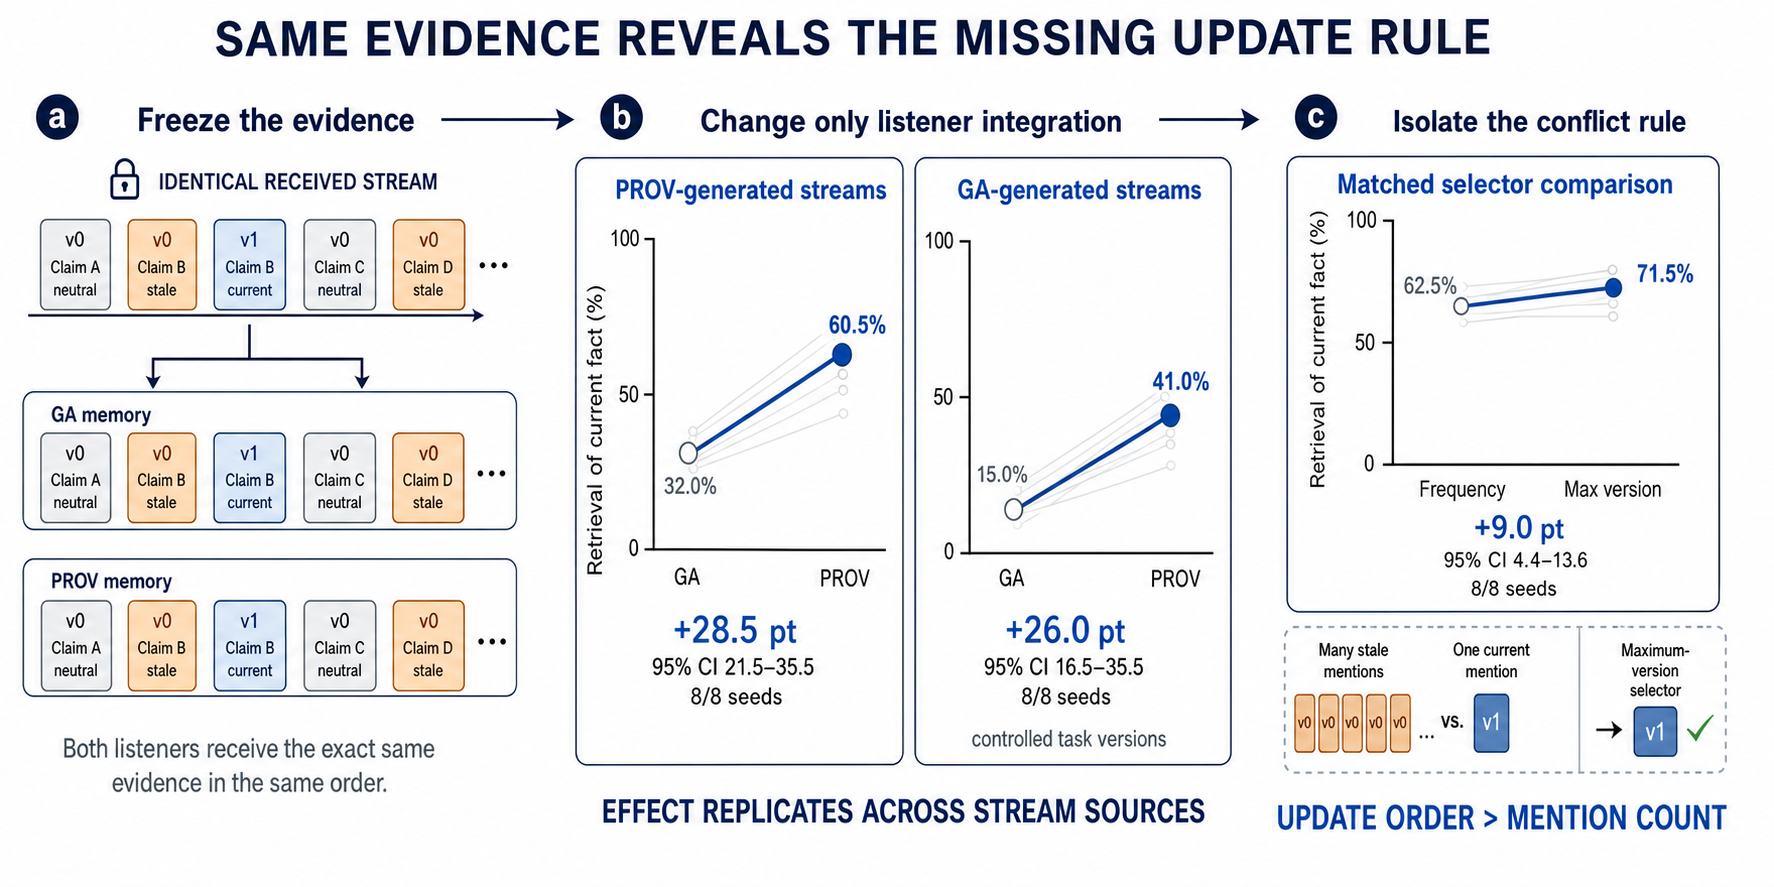
\includegraphics[width=\textwidth,trim=0 0 0 75,clip]{story_redesign/fig2_causal_chain_v1.png}
  \caption{Same evidence, different memory.  \textbf{a}, Both pipelines receive the same ordered
  stream.  \textbf{b}, Complete \prov{} integration improves current \held{} across both stream
  sources.  \textbf{c}, With all other operations fixed, maximum-version selection outperforms
  mention frequency.  All paired effects are positive in eight of eight seeds; intervals are
  shown in the panels.}
  \Description{A frozen received stream is copied into GA and provenance-aware listener memories.
  Two paired comparisons show positive complete-pipeline gains on independently generated stream
  sources.  A final matched comparison isolates a smaller positive effect of maximum-version
  selection over mention frequency.}
  \label{fig:nested}
\end{figure*}

The public--private mismatch alone does not identify where the update is lost.  Exposure predicts
success within a condition: agents that hear a larger share of current mentions
are more likely to return the current answer.  Across conditions, however, mean current
heard-fractions are similar (0.64 baseline, 0.72 source, 0.73 broadcast) while \held{} outcomes are
opposite (12\%, 15\%, 99\%).  Received frequency therefore underdetermines the final answer.

Matched-event replay provides the causal contrast.  On identical text-plus-metadata streams,
\ga{} reaches 32.0\% current \held{} answers (95\% CI 28.0--36.0), whereas \prov{} reaches 60.5\%
(52.8--68.2).  The paired gain is 28.5 percentage points (21.5--35.5).  It is positive in all
eight schedule seeds; the exact two-sided sign test gives $p=.0078$.  Since both memories receive
the same event sequence, architecture-induced differences in later conversation cannot explain
this replay gap.  The result identifies listener-side \emph{memory handling} as causally
consequential under structured provenance: changing what a listener does with the same evidence
changes what it can later return.  Because the pipelines also differ in representation,
consolidation, retrieval, and context salience, this 28.5-point contrast does not by itself assign
the gain to one rule (Figure~\ref{fig:nested}b).

A complementary cross-source replay uses eight realized \ga{} society streams.  Because those
transcripts contain no native metadata, the controlled task supplies version 1 to unambiguous
current mentions and version 0 to unambiguous stale mentions; mixed claims remain unannotated.
On these identical text-plus-annotation streams, \ga{} reaches 15.0\% current answers and \prov{}
41.0\%, a paired gain of 26.0 points (95\% CI 16.5--35.5; positive in 8/8 seeds; exact sign test
$p=.0078$).  The listener effect therefore persists beyond \prov{}-generated linguistic support,
conditional on correct task versions; it does not validate automatic provenance extraction.

\subsection{Version priority, not repetition, resolves one conflict mechanism}

The strict matched-policy ablation makes that assignment at a smaller scale.  With every other
operation held isomorphic, mention-frequency selection yields 62.5\% current answers (95\% CI
52.7--72.3), while maximum-version selection yields 71.5\% (64.3--78.8).  The paired difference
is +9.0 points (4.4--13.6), positive in all eight seeds (exact two-sided sign test $p=.0078$).
The 400 common-prompt interviews exactly match the selected symbolic state.  Thus, supplied
version priority itself has a positive causal effect; the remainder of the larger pipeline gap
may arise from representation, retrieval salience, consolidation, or their interactions
(Figure~\ref{fig:nested}c).

\paragraph{Two mechanisms}

The complete-pipeline and selector-only interventions improve different failure modes.  In the complete
pipeline comparison, \prov{} produces 121 current, 10 stale, and 69 unknown answers over 200
agents; \ga{} produces 64 current, 15 stale, and 121 unknown.  The 57 additional current answers
are therefore accompanied mainly by 52 fewer unknowns rather than by a large stale-to-current
conversion.  This pattern is consistent with explicit retrieval salience: once a versioned update
reaches an agent, \prov{} places the selected state at the top of the interview context instead of
asking the model to resolve a mixed event/reflection set.  The paired gain in the net
current-minus-stale rate is 31.0 points (95\% CI 25.1--36.9).

The selector-only ablation has a sharper signature.  Both policies leave the same 23 agents
unknown because neither changes reach or candidate extraction.  Maximum-version selection converts
18 outcomes from stale to current relative to frequency, changing pooled counts from
125/52/23 to 143/34/23.  Seed 46 supplies the largest contrast: five agents receive a numerical
majority of stale mentions after at least one version-1 update, so frequency returns stale while
maximum version returns current.  The fact that unknown is invariant in this ablation helps rule
out retrieval volume or interview compliance as the explanation for its 9-point gain.  This is
the paper's narrow mechanistic result: for a received mutable fact, order in the version sequence
can matter more than popularity in the transcript.

\subsection{The repair persists across controlled settings}

Under one social harness, raw transcript storage reaches 14\%; controlled Mem0, A-MEM, and
MemoryBank adaptations, \ga{}, and a
current-focused \ga{} variant range from 18\% to 25\%.  \prov{} reaches 57\%.  The comparison
should be read as a mechanism test, not a leaderboard: all adaptations share our simulator,
prompts, and interface rather than reproducing each external system end to end.

The advantage persists beyond the repair-drive wording.  Across three scenarios, current
\held{} is \prov{}/\ga{} = 57/22 for a repair drive, 69/47 for a book club, and 59/18 for a
carpool.  A numeric dues change gives 59\% versus 28\%.  These scenario and fact-type checks use
five seeds except the eight-seed repair-drive architecture cell; their intervals are reported in
Table~\ref{tab:generality}.  At round 10, random, ring, and small-world point estimates are 93/22,
68/6, and 83/10.  On a second model family, DeepSeek-V4-Flash, the eight-seed comparison is
64.0\% \prov{} versus 15.5\% \ga{} with disjoint intervals.  Five-seed official-API
coverage of the remaining memory rows ranges from 13.6\% to 39.2\%; none closes the gap
to \prov{}.

\begin{table*}[t]
  \caption{Memory comparison at a glance.  Entries are current \held{} (\%); brackets are
  seed-level 95\% intervals.  Bold and underline mark the best and second-best multi-seed,
  non-ceiling results.  Dashes are not scheduled or not applicable.  Named systems are
  controlled motif adaptations, not official implementations.}
  \label{tab:generality}
  \centering
  \footnotesize
  \renewcommand{\arraystretch}{1.15}
  \begin{tabular*}{\textwidth}{@{\extracolsep{\fill}}lccccccc c cc@{}}
    \toprule
    & \multicolumn{7}{c}{Current \held{} across tasks and settings} &
      \multicolumn{1}{c}{Summary} & \multicolumn{2}{c}{Update interface} \\
    \cmidrule(lr){2-8}\cmidrule(lr){9-9}\cmidrule(l){10-11}
    Memory & \shortstack{Repair\\drive} & \shortstack{Book\\club} & Carpool &
      \shortstack{Numeric\\dues} & \shortstack{Three-step\\update} &
      \shortstack{Long horizon\\($r=10$)} & \shortstack{DeepSeek\\V4-Flash} &
      \shortstack{Mean $r=5$\\$\uparrow$\textsuperscript{\S}} &
      \shortstack{Explicit\\version} & \shortstack{Relays\\source} \\
    \midrule
    Raw transcript & \cellci{14}{6,23} & \cellci{28}{0,56} &
      \cellci{11}{0,31} & \cellci{16}{0,35} & \cellci{10}{1,20} &
      \cellci{8}{0,30} & \cellci{\underline{39.2}}{27.3,51.1} & 17.4 & no & no \\
    Mem0 motif & \cellci{18}{14,23} & \cellci{\underline{66}}{29,100} &
      \cellci{19}{10,28} & \cellci{22}{8,37} & \cellci{\underline{19}}{1,37} &
      \cellci{30}{0,80} & \cellci{26.4}{16.1,36.7} & \underline{31.4} & no & no \\
    A-MEM motif & \cellci{19}{12,26} & \cellci{52}{38,66} &
      \cellci{\underline{30}}{25,34} & \cellci{25}{20,30} &
      \cellci{14}{3,26} & \cellci{18}{0,37} & \cellci{30.4}{12.3,48.5} &
      \underline{31.4} & no & no \\
    \ga{} & \cellci{22}{13,30} & \cellci{47}{45,49} & \cellci{18}{10,25} &
      \cellci{\underline{28}}{18,38} & \cellci{18}{8,27} & \cellci{22}{15,28} &
      \cellci{15.5}{10.1,20.9} & 28.5 & no & no \\
    Current-focused \ga{} & \cellci{\underline{25}}{15,35} &
      \cellci{42}{17,67} & \cellci{24}{17,31} & \cellci{8}{1,15} &
      \cellci{8}{1,15} & \cellci{\underline{33}}{13,53} &
      \cellci{13.6}{5.3,21.9} & 24.6 & no & no \\
    MemoryBank motif & \cellci{\underline{25}}{19,31} & \cellci{42}{4,81} &
      \cellci{18}{4,33} & \cellci{27}{19,35} & \cellci{11}{3,19} &
      \cellci{13}{0,28} & \cellci{26.4}{15.0,37.8} & 28.2 & no & no \\
    \midrule
    \textbf{\prov{} (ours)} & \cellci{\textbf{57}}{49,65} &
      \cellci{\textbf{69}}{62,76} & \cellci{\textbf{59}}{49,69} &
      \cellci{\textbf{59}}{49,69} & \cellci{\textbf{68}}{59,77} &
      \cellci{\textbf{93}}{82,100} &
      \cellci{\textbf{64.0}}{57.8,70.2} & \textbf{61.0} &
      \textbf{yes} & \textbf{yes} \\
    \addlinespace
    Broadcast ceiling & \cellci{99}{97,100} & -- & -- & -- & -- & -- & -- &
      -- & n/a & n/a \\
    \bottomrule
  \end{tabular*}
  \vspace{2pt}

  {\scriptsize Three-step uses three successive updates and three full post-final-update
  propagation rounds ($r=7$); long-horizon uses $r=10$.
  \textsuperscript{\S}Mean $r=5$ is the equal-weight macro-average of Repair drive,
  Book club, Carpool, and Numeric dues; $r=7$, $r=10$, and DeepSeek cells are excluded.
  Long-horizon \ga{} uses the eight-seed C17 reference and long-horizon \prov{} uses five
  seeds.  DeepSeek \ga{} and \prov{} use eight seeds; the other DeepSeek cells use five
  official-API seeds.}
\end{table*}

These checks broaden the observed pattern but do not turn the controlled probe into a universal
claim.  Scenario surfaces share the same change-and-propagate structure, topology cells are
point-estimate robustness checks, and only two model families are included.

\subsection{Provenance is the missing interface between speech and memory}

\begin{figure*}[t]
  \centering
  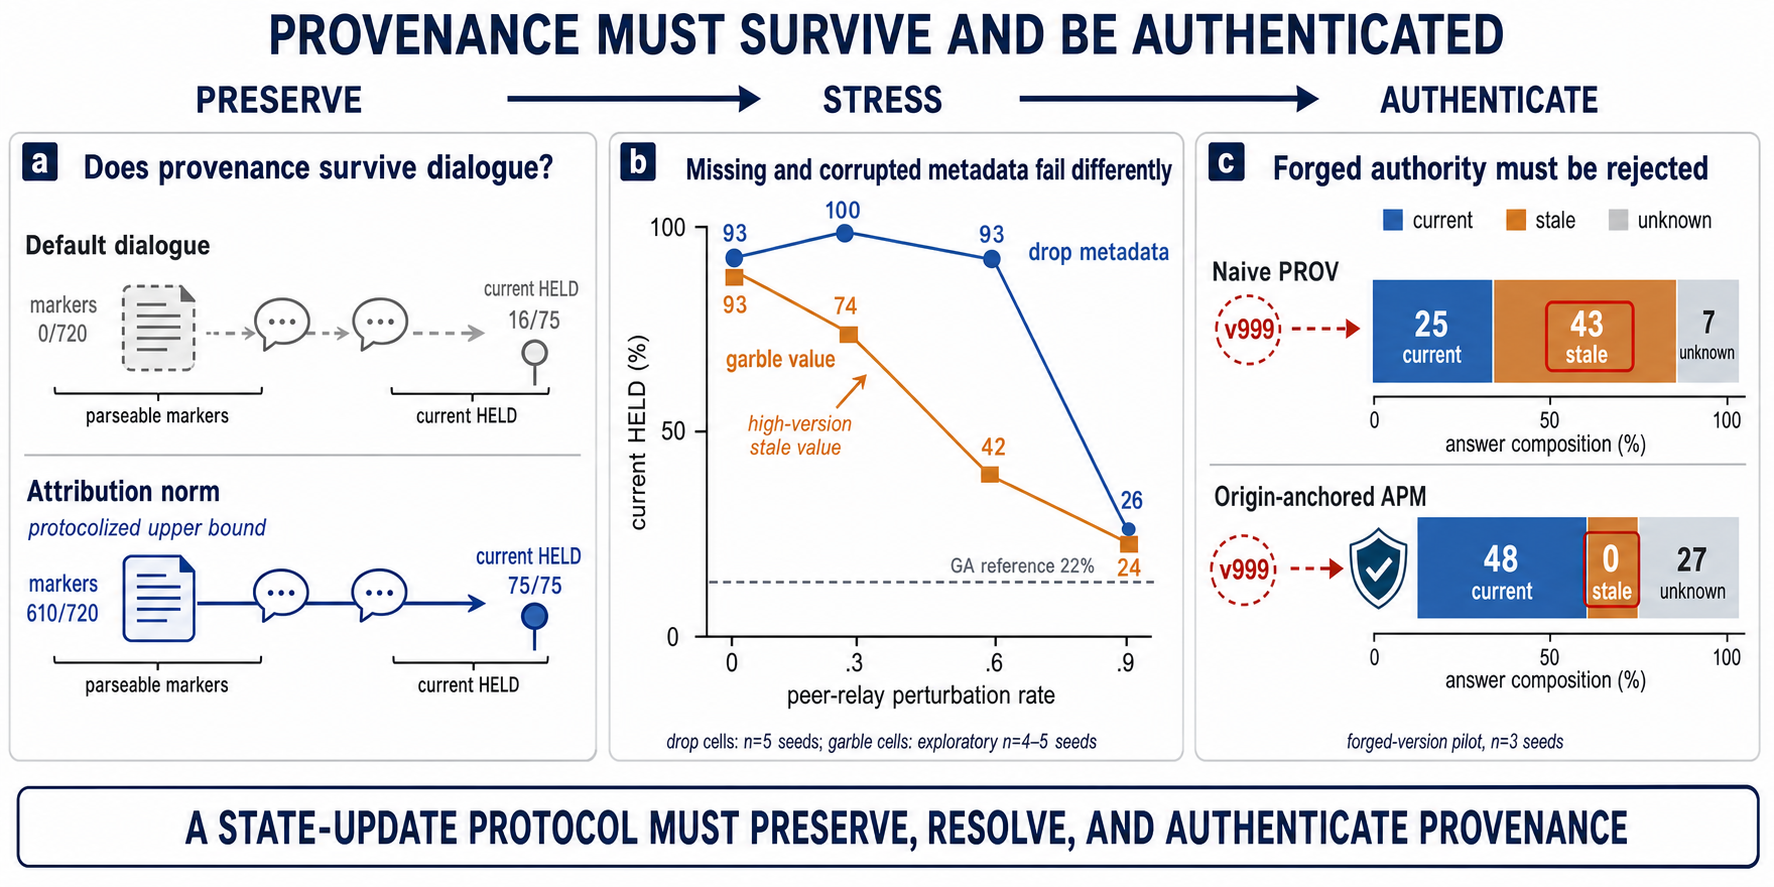
\includegraphics[width=0.95\textwidth,trim=0 120 0 65,clip]{story_redesign/fig3_protocol_boundary_v1.png}
  \caption{Provenance needs a protocol.  \textbf{a}, Default dialogue preserves
  few usable markers; explicit attribution preserves them.  \textbf{b}, Missing metadata degrades
  gradually, whereas corrupted high-version values mislead.  \textbf{c}, Origin anchoring rejects
  the tested forged version that naive \prov{} accepts.  Counts and sample sizes are shown in the
  panels.}
  \Description{A three-stage protocol chain shows provenance preservation in text-only dialogue,
  current-answer rates under dropped and corrupted metadata, and current, stale, and unknown
  outcomes under a forged high-version attack with and without origin anchoring.}
  \label{fig:boundaries}
\end{figure*}

The structured intervention identifies what a reliable interface can do, but deployment also
requires provenance to reach the interface.  We test this dependency with text-coupled memory at
round 10.  Under default LLM dialogue, only 16 of 75 agents return the current value; none return
the stale value, and 59 abstain as unknown.  More importantly, zero of 720 utterances preserves a
source/version phrase, so the provenance parser has almost nothing to integrate.  Under a strong
attribution norm, 610 of 720 utterances contain source/version-like markers and all 75 agents
return the current value.  The norm uses natural-language text rather than hidden event fields,
but its strength makes it a protocolized upper bound rather than ordinary conversation
(Figure~\ref{fig:boundaries}a).

These results separate two requirements that an end-to-end score would conflate:
communication must preserve provenance, and the listener must integrate it.  The matched-event
replay establishes the second requirement conditional on the first; this text-only contrast
shows why the first cannot be assumed.  Provenance-aware memory is therefore not a self-contained
repair.  It is one endpoint of a state-update interface spanning communication and memory.

\subsection{Missing metadata degrades; corrupted metadata misleads}

Structured metadata need not be perfectly transmitted to be useful, but corrupt metadata is more
dangerous than missing metadata.  We stress the round-10 repair-drive system with two independent
per-relay perturbations.  Under \emph{drop}, the provenance payload is absent while the ordinary
utterance is still delivered.  Under \emph{garble}, the payload keeps its high version but carries
the stale value.  The authoritative source's direct receipt is never perturbed.  Drop cells use
five seeds; garble cells use four or five and are treated as exploratory point estimates.

Figure~\ref{fig:boundaries}b shows redundancy under missing metadata: current answers remain
93--100\% through 60\% drop, then approach the \ga{} reference at 90\% drop.  Garbling degrades
more steadily because naive \prov{} treats a stale value with a high version as authoritative.
At 60\% garble it retains 42\% current, but at 90\% it is indistinguishable from the 22\% \ga{}
reference at the precision of this exploratory check.  These cells address the narrow objection
that every relay must be lossless; they do not model correlated failure or an adaptive attacker.

The stress test also exposes a design defect.  Once a garbled value is stored at version $z$, a
later correct claim at the same version cannot replace it because the update rule requires
$z_e>z_i$.  A deployed protocol therefore needs same-version conflict handling rather than
first-arrival stickiness: retain both candidates, validate the origin signature and content hash,
or abstain until independent paths agree.  The origin-anchored extension below addresses forged
authority, but its small pilot does not exhaust these conflict cases.

\subsection{Authentication turns provenance into a protocol}

\prov{} adopts the highest version blindly.  An adversary can therefore attach a forged version
999 to the stale value.  We harden the protocol into Auditable Provenance Memory (\apm{}) with
three mechanisms: (1) an authorization flag minted only at the origin and relayed without
escalation; (2) a source--version--path trace retained with every candidate; and (3) optional
independent-path corroboration before commitment, with abstention represented as unknown.
These mechanisms make each accepted update auditable and prevent an ordinary speaker from
manufacturing origin authority.

In a three-seed, model-matched pilot, the forged stale claim leaves \prov{} at 33\% current and
raises stale answers to 57\% (43 of 75 agents).  Under the same attack, \apm{} yields 64\%
current with no stale answer among 75 agents (Figure~\ref{fig:boundaries}c).  This is evidence for
the specific defense against the specific attack, not a general adversarial guarantee.  A separate
sparse-communication check ($n=8$, round 10) yields 40.5\% current for \apm{} and 21.5\% for
\ga{} with overlapping current-answer intervals; the clearer safety difference is stale 0/200
for \apm{} versus 30/200 for \ga{}.  We therefore treat \apm{} as a promising hardening extension,
not the paper's primary efficacy claim.

\section{Discussion}

\paragraph{The transcript is not the society's state}
Public speech moved toward the update while population retrieval showed no supported gain, so a
corrected-looking transcript did not establish a corrected society.  Because \said{} and
\held{} have different observational units, this is not evidence that most agents said the
update and then forgot it.  It is a gap between public visibility and population retrieval;
evaluations should measure both rather than treating the first as a proxy for the second.

\paragraph{Mutable facts are state transitions, not votes}
Fixed-stream interventions turn the observational gap into a diagnosis: changing listener-side
handling of the same evidence changed later answers.  The matched selector isolated a 9.0-point
benefit from maximum-version priority, supporting a specific principle: once a mutable fact
reaches a listener, conflict resolution should respect update order rather than only repetition.
This rule does not explain the entire 28.5-point pipeline gain; state salience, consolidation, and
retrieval remain candidate mechanisms.

\paragraph{The repair is a protocol, not a memory module}
Version-aware selection works only when communication supplies trustworthy versions.  Default
dialogue preserved no parseable source/version marker, and corrupted high-version metadata could
install a stale value.  A reliable interface must therefore connect reach, preservation,
resolution, and authentication, with abstention when any stage fails
(Appendix~\ref{app:extended-boundaries}).  This systems layer---not provenance storage
alone---is the broader implication of the repair.

\paragraph{Scope and alternatives}
The experiments establish the value of correct provenance at one listener-side locus, not that
integration is the only source of the gap or that deployed agents will infer trustworthy metadata
automatically.  The study covers 25-agent, short-horizon event tasks and few model families;
\held{} is elicited behavior, replays assume structured or controlled-task versions, and the
\apm{} pilot is not a security certification.  Provenance interfaces also trade naturalism for
auditability and may be unsuitable when provenance loss is itself under study.

\section{Ethical and Social Considerations}

The study uses synthetic personas and no human data.  Provenance can improve auditability but may
also enable surveillance or misplaced trust in credentials; deployment requires data minimization,
credential protection, uncertainty disclosure, and stakeholder validation.  Generative AI tools
assisted coding, search, checks, and revision; the authors inspected the outputs.

\section{Conclusion}

A fact can win the conversation without updating the society.  Separating \heard{}, \said{}, and
\held{} exposed that failure, while fixed-evidence replays located a consequential part of it in
listener-side integration.  Provenance-aware memory gained 28.5 points on identical streams, and
the stricter selector intervention isolated a 9.0-point benefit from version priority over
repetition.  The resulting design lesson is bounded but concrete: mutable facts in LLM agent
societies need a provenance-preserving, authenticated state-update interface between
communication and memory, and evaluation must test retrievable state rather than infer it from
public speech.

\clearpage
\bibliographystyle{ACM-Reference-Format}
\bibliography{references}

\clearpage
\appendix

\section{Reproducibility and Artifact Map}
\label{app:repro}
\label{app:reproduction}

The anonymous artifact contains the simulator, memory code, prompts, replay scripts, aggregation
scripts, normalized selector records, per-seed outputs, run configurations, a sanitized execution
provenance record, and a data index.
Core transcripts are included, while aggregate-only exploratory cells are labeled.  Model
identifiers and access-time configurations are recorded, but proprietary weights and provider
infrastructure cannot be archived; fresh generations may therefore differ.

Three reproduction levels separate model-free checks from new generation.  Headline numbers
re-aggregate offline from accepted per-agent and per-seed JSON.  The fixed-stream runner
reconstructs eight societies, comprising 200 per-agent streams, and verifies every terminal
version--value pair against the saved \prov{} snapshot before any model call.  The selector
runner reproduces normalization, outcomes, intervals, and exact sign tests offline; its online
mode repeats the common-prompt interviews.  Expected aggregates and a SHA-256 package manifest
are included.

The schedule seed controls pairings and topology sampling but cannot make proprietary model
generation bitwise deterministic.  Saved accepted runs are therefore the evidential record, and
each condition must contain all 25 agents.  Reproduction proceeds by (1) verifying the manifest
and environment lock; (2) re-aggregating accepted JSON; (3) reconstructing the eight societies
and checking 200 terminal agent states; (4) rerunning selector normalization, intervals, and
sign tests; and, optionally, (5) repeating interviews or full society generation.  A missing
agent, failed state check, or unregistered seed--configuration pair causes the corresponding
condition to fail closed.

\begin{table}[!ht]
  \caption{Claim-to-artifact map.}
  \label{tab:app-artifacts}
  \centering
  \small
  \begin{tabular}{@{}p{2.3cm}p{4.7cm}@{}}
    \toprule
    Claim family & Required records \\
    \midrule
    \said{}/\held{} gap & final-round logs, interviews, marker and semantic-judge audit \\
    Complete replay & ordered observations, memory snapshots, replay checkpoints \\
    Cross-source replay & \ga{} streams, task annotations, paired checkpoints \\
    Selector effect & normalized candidates, policy outputs, paired seed summaries \\
    Text preservation & utterance logs and source/version marker audit \\
    Channel stress & corruption configuration and accepted interviews \\
    Forged version & attacker configuration, origin checks, final verdicts \\
    \bottomrule
  \end{tabular}
\end{table}
\FloatBarrier

\section{Extended Implications and Boundaries}
\label{app:extended-boundaries}

\paragraph{Nested causal estimands}
\label{app:causal-scope}
The comparisons answer different questions.  End-to-end communication is endogenous: a memory
that changes one speaker's context can alter downstream evidence.  Primary fixed-event replay
removes that feedback but conditions on \prov{}-generated streams and combines all local pipeline
differences.  Cross-source replay repeats the pipeline contrast on \ga{} text while supplying
oracle task versions.  Selector-only replay is more causally specific because it fixes local
representation and prompting, but it too assumes correct annotations.

\begin{table}[!ht]
  \caption{Nested comparisons and the claims they support.}
  \label{tab:estimands}
  \centering
  \small
  \begin{tabular}{@{}p{1.5cm}p{1.75cm}p{3.55cm}@{}}
    \toprule
    Comparison & Held fixed & Supported estimand \\
    \midrule
    End to end & task, model, schedules & Total interface effect; dialogue may mediate \\
    Fixed event & received stream & Conditional pipeline effect on \prov{} support \\
    Cross source & \ga{} text, task versions & Conditional pipeline effect beyond \prov{} text \\
    Selector only & candidates, context, interview & Maximum version versus frequency \\
    \bottomrule
  \end{tabular}
\end{table}

\paragraph{Four-stage reliability chain}
The experiments separate four requirements that a monolithic ``memory quality'' score would
hide.  First, the update must \emph{reach} the listener: provenance reaches only 10--19 agents in
the primary fixed streams, and the lowest-coverage seed has the smallest complete-pipeline lift.
Second, metadata must \emph{survive} communication: default text-only dialogue preserves no
parseable source/version marker in 720 utterances, whereas an explicit norm preserves 610.
Third, the listener must \emph{resolve} conflicts using that metadata: maximum-version selection
gains 9.0 points over mention frequency.  Fourth, metadata must be \emph{authenticated}: a forged
version 999 hijacks naive \prov{}, while origin anchoring rejects the tested unauthenticated claim.

\paragraph{Interface fallbacks}
Failure of reach should produce unknown rather than an invented current value.  Failed
preservation should trigger a request for metadata or direct source confirmation.  Same-version
conflicts should remain unresolved until corroborated, and failed authentication should
quarantine the claim rather than merely lower its textual relevance.  Such interfaces are useful
for auditable coordination but may be undesirable in descriptive social simulations, where
selective absorption and provenance loss are behaviors to reproduce.

\begin{table}[!ht]
  \caption{Natural levers do not provide a reliable repair.  Brackets are seed-level 95\%
  intervals where reported; values without intervals are exploratory point estimates.}
  \label{tab:levers}
  \centering
  \small
  \begin{tabular}{@{}lp{1.9cm}p{3.9cm}@{}}
    \toprule
    Lever & Conditions ($n$) & Current \held{} (\%) \\
    \midrule
    Capability & mini / 5.4 / 5.5 (8/5/5) & 18 [12,25] / 34 [25,44] / 30 [21,40] \\
    Connectivity & 1 / 2 / 3 meetings (8 each) & 20 [13,26] / 18 [12,25] / 14 [10,18] \\
    Persona & thin / rich (5 each) & 12 / 14 \\
    Authority & base / source (5 paired) & 12 [3,21] / 15 [10,21] \\
    Memory motifs & Raw--MemoryBank (8 each) & 14--25 \\
    Positive control & overwrite (5) & 99 [97,100] \\
    \bottomrule
  \end{tabular}
\end{table}

\paragraph{Scope and ethical boundary}
The harness is a 25-agent, short-horizon simulation over event-planning facts and few model
families; it does not cover negotiation, strategic deception, multi-hop planning, or real users.
Exploratory long-horizon cells are underpowered.  The primary replay conditions on
\prov{}-generated support, while the cross-source and selector tests use oracle task annotations.
Controlled adaptations are not official system benchmarks, the semantic audit covers only the
375 core interviews, and the three-seed \apm{} pilot does not establish robustness to forged
origins, compromised sources, collusion, replay, or path manipulation.

The study contains no human participants, private records, or demographic inference.  Its risks
are dual use, anthropomorphic over-interpretation, surveillance through provenance traces, and
misplaced trust in credentials.  Deployment should minimize retained content, protect and rotate
credentials, expose uncertainty and abstention, and undergo stakeholder validation.

\section{Task, Measures, and Memory Contract}
\label{app:task}
\label{app:memory}

\subsection{Registered task state and exposure}
\label{app:exposure}

The principal repair-drive scenario registers exactly two admissible event states:
\[
  \begin{aligned}
  v_0 &= \text{Saturday at the front porch},\\
  v_1 &= \text{Sunday at the community center}.
  \end{aligned}
\]
The environment initializes agents with $v_0$ and injects $v_1$ into the designated source after
the first round's encounters.  The book-club, carpool, and dues checks preserve the same
one-change structure but substitute scenario-specific values.  Marker classifiers receive the
registered pair for that scenario; they do not search for arbitrary world knowledge.

For agent $i$, let $E_{qri}=(e_{qri1},\ldots,e_{qrim_{qri}})$ be the events delivered in arrival
order.  Using the predicates from Section~3.2, current reach and current-marker composition are
\[
 R_{qri}=\mathbb{1}\!\left[\sum_j\mathbb{1}[C(e_{qrij})]>0\right],
 \qquad
 D_{qri}=
 \frac{\sum_j\mathbb{1}[C(e_{qrij})]}
      {\sum_j\mathbb{1}[V(e_{qrij})]}.
\]
$D_{qri}$ is undefined when no value-bearing event was received; aggregate summaries report the
number of agents with a defined denominator.  These diagnostics describe input exposure and do
not treat receipt as adoption.

\begin{table}[!ht]
  \caption{Core execution contract.}
  \label{tab:app-contract}
  \centering
  \small
  \begin{tabular}{@{}ll@{}}
    \toprule
    Item & Registered setting \\
    \midrule
    Society size & 25 agents \\
    Transmission horizon & 5 rounds unless stated otherwise \\
    Meeting density & 2 pairwise meetings per agent per round \\
    Meeting length & 3 alternating utterances \\
    Independent unit & schedule seed \\
    Core paired seeds & 41--48 \\
    Primary generator & \texttt{gpt-5.4-mini}, temperature 0 \\
    Model-family check & \texttt{DeepSeek-V4-Flash} \\
    Interview output & one JSON sentence, read-only \\
    Verdicts & current, stale, unknown \\
    \bottomrule
  \end{tabular}
\end{table}

\subsection{Prompt contract}

The conversation system message is:
\begin{quote}\small\ttfamily\raggedright
You are role-playing a person in a small neighborhood. Stay in character and stay consistent
with your memory notes - only act on what is currently true and honor any commitments you have
made. Reply with ONE short, natural utterance (1-2 sentences). Return ONLY JSON:
\{"utterance": "..."\}
\end{quote}
The conversation user message supplies the speaker persona, listener, topic, retrieved memory
notes, optional communication norm, prior utterances in that meeting, and the question
``What does [speaker] say next?''  The default prompt does not request a source or version; the
strong-attribution condition adds that requirement explicitly.

The interview system message is:
\begin{quote}\small\ttfamily
Answer the question using ONLY the memory notes, reflecting the CURRENT state. Reply with one
short sentence. Return ONLY JSON: \{"answer": "..."\}
\end{quote}
The interview call cannot modify memory, and no subsequent conversation occurs.  Thus \held{} is
elicited from the final retrieval context rather than self-reported during transmission.

\subsection{Memory interfaces}

Every observed utterance has an immutable arrival index, round, speaker, listener, and text.
Structured conditions may additionally carry an origin, version, and typed value.  The raw log
is retained even when a memory maintains a compact derived state, allowing the audit to separate
what arrived from what the memory accepted.

The \ga{} adaptation appends observed events, produces up to three free-text reflections at round
boundaries from the ten most recent events, and retrieves six events plus three reflections for
the interview.  The \prov{} pipeline appends the same raw events and maintains a pair
$(z_i,v_i)$ initialized to $(0,v_0)$.  For each typed claim $(z_e,v_e)$, it replaces that pair
only when $z_e>z_i$.  Retrieval prepends the accepted pair and returns four relevance-ranked raw
events.  This complete-pipeline contrast therefore includes representation, consolidation,
selection, retrieval budget, and salience.

The stricter ablation creates a common candidate multiset
\[
 C_i=\{(a_k,z_k,v_k):k=1,\ldots,m_i\},
\]
where $a_k$ is the arrival index.  Both policies use the same store, no-op consolidation,
one-record retrieval budget, context string, model call, and verdict function.  The frequency
policy returns the value with the largest candidate count and breaks ties by latest arrival; the
version policy returns the candidate with largest $z_k$ and uses the same tie break.

\begin{table}[!ht]
  \caption{Controlled operations in the selector-only ablation.}
  \label{tab:app-isomorphic}
  \centering
  \small
  \begin{tabular}{@{}lll@{}}
    \toprule
    Operation & Frequency & Maximum version \\
    \midrule
    Candidate schema & identical & identical \\
    Candidate multiset & identical & identical \\
    Consolidation & no-op & no-op \\
    Retrieval budget & one record & one record \\
    Context template & identical & identical \\
    Interview/scorer & identical & identical \\
    Conflict rule & count, then arrival & version, then arrival \\
    \bottomrule
  \end{tabular}
\end{table}
\FloatBarrier

\section{Replay Construction and Paired Evidence}
\label{app:reconstruction}
\label{app:paired}

For each seed, the replay builder reads the accepted round logs, expands every meeting into
ordered listener observations, and sorts them by round and arrival index.  It checks the
reconstructed terminal version and value of each agent against the saved \prov{} snapshot; a
mismatch aborts replay.  Across the eight societies, the normalization audit partitions 5,412
received events into 494 structured provenance candidates, 556 unambiguous text-derived
candidates, 40 ambiguous mentions excluded from selection, and 4,322 events containing neither
registered value.  Text-derived versions are analysis annotations based on the registered
$v_0/v_1$ pair, not evidence of natural-language provenance extraction.

\begin{figure}[!ht]
  \centering
  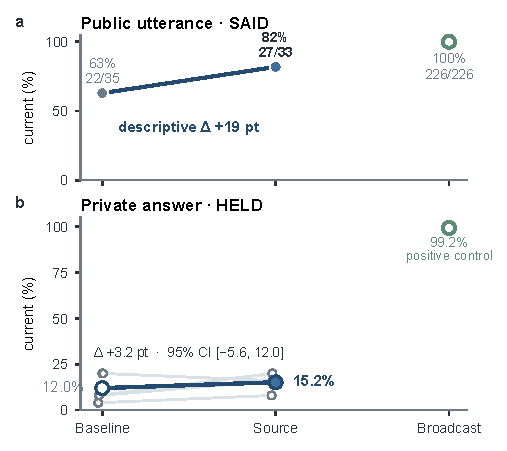
\includegraphics[width=\columnwidth]{final_redesign/exports/fig2_dissociation.pdf}
  \caption{Public uptake, weak retrieval.  \textbf{a}, Pooled public current mentions increase
  under a persistent source.  \textbf{b}, Paired private answers remain near baseline.  Broadcast
  is an overwrite positive control; points, intervals, and sample sizes are shown in the panels.}
  \Description{Two panels compare baseline, persistent-source, and broadcast conditions.
  Public current utterances increase under the source condition, while paired private-answer
  rates remain near baseline; broadcast is near 100 percent on both measures.}
  \label{fig:sayhold}
\end{figure}
\FloatBarrier

\begin{table*}[!t]
  \caption{Per-seed current \held{} rates for three paired replay experiments.  Each seed cell
  is a percentage over 25 agents.  The pooled rows report verdict counts over 200 agents per
  policy; all 400 selector interviews matched the selected symbolic state.}
  \label{tab:app-replay-seeds}
  \label{tab:app-selector-seeds}
  \centering
  \small
  \begin{tabular}{@{}llrrrrrrrrr@{}}
    \toprule
    Replay & Policy & 41 & 42 & 43 & 44 & 45 & 46 & 47 & 48 & Mean \\
    \midrule
    Complete pipeline & \ga{} & 36 & 36 & 24 & 28 & 28 & 36 & 36 & 32 & 32.0 \\
                      & \prov{} & 72 & 64 & 64 & 60 & 40 & 60 & 64 & 60 & 60.5 \\
                      & Difference & 36 & 28 & 40 & 32 & 12 & 24 & 28 & 28 & 28.5 \\
    \addlinespace
    \ga{}-source pipeline & \ga{} & 32 & 20 & 16 & 16 & 8 & 12 & 12 & 4 & 15.0 \\
                         & \prov{} & 56 & 52 & 60 & 48 & 40 & 20 & 28 & 24 & 41.0 \\
                         & Difference & 24 & 32 & 44 & 32 & 32 & 8 & 16 & 20 & 26.0 \\
    \addlinespace
    Selector only & Mention frequency & 72 & 68 & 80 & 68 & 52 & 44 & 60 & 56 & 62.5 \\
                  & Maximum version & 76 & 76 & 84 & 76 & 56 & 64 & 72 & 68 & 71.5 \\
                  & Difference & 4 & 8 & 4 & 8 & 4 & 20 & 12 & 12 & 9.0 \\
    \bottomrule
  \end{tabular}

  \vspace{3pt}
  \begin{tabular}{@{}llrrr@{}}
    \toprule
    Replay & Policy & Current & Stale & Unknown \\
    \midrule
    Complete pipeline & \ga{} / \prov{} & 64 / 121 & 15 / 10 & 121 / 69 \\
    \ga{}-source pipeline & \ga{} / \prov{} & 30 / 82 & 16 / 38 & 154 / 80 \\
    Selector only & Frequency / version & 125 / 143 & 52 / 34 & 23 / 23 \\
    \bottomrule
  \end{tabular}
\end{table*}

Both complete-pipeline comparisons improve all eight seeds.  On \prov{}-generated streams, the
listener change shifts 57 pooled answers to current, primarily by reducing unknown outcomes.  On
\ga{}-generated streams, it shifts 52 to current but also 22 to stale when only version-0 evidence
is available; its net current-minus-stale interval crosses zero.  The selector-only comparison improves all
eight seeds but leaves unknown fixed at 23 and converts 18 stale outcomes to current.  These
distinct error signatures support the nested interpretation in the body: version priority is
one verified component, while explicit state representation and retrieval salience contribute
additional pipeline-level benefit.
\FloatBarrier

\section{Robustness and Security Boundaries}
\label{app:robustness}
\label{app:attack}

Scenario, fact-type, topology, and model-family results are reported once, in
Table~\ref{tab:generality}.  The remaining diagnostics test whether provenance survives the
communication channel and whether a larger version number can be forged.

\begin{table}[H]
  \caption{Channel and security boundary diagnostics.}
  \label{tab:app-boundaries}
  \label{tab:app-text}
  \label{tab:app-stress}
  \label{tab:app-attack}
  \centering
  \small
  \begin{tabular}{@{}llrrr@{}}
    \toprule
    Test & Condition & Current & Stale & Unknown \\
    \midrule
    Text only & Default & 16 & 0 & 59 \\
              & Strong attribution & 75 & 0 & 0 \\
    \addlinespace
    Channel stress & Metadata drop & 93/100/93/26 & -- & -- \\
                   & Value garbling & 93/74/42/24 & -- & -- \\
    \addlinespace
    Forged version & Naive \prov{} & 25 & 43 & 7 \\
                   & \apm{} & 48 & 0 & 27 \\
    \bottomrule
  \end{tabular}
  \par\medskip
  \parbox{\columnwidth}{\footnotesize Text-only and forged-version rows give pooled
  current/stale/unknown counts.  Stress-test current counts correspond to
  $p=0.0/0.3/0.6/0.9$, each out of 100.  Default and strong-attribution dialogue preserve
  0/720 and 610/720 marked utterances.}
\end{table}

Default text-only dialogue preserves no parseable source--version marker, and most agents
abstain.  A strong attribution norm preserves 610 of 720 markers and provides an
upper bound under protocolized communication.  Metadata drop is partly masked by redundant
paths, whereas value garbling degrades current answers more steadily because a high version can
carry the stale value.  These finite-run cells are diagnostics rather than monotonicity
estimates.

Naive \prov{} treats a larger integer as authoritative.  The forged-version pilot therefore
gives one relayer an unauthenticated stale claim labeled version 999.  The origin-anchored
extension \apm{} accepts a versioned update only when its origin matches the registered authority
and retains the relay path for audit.  It does not claim cryptographic security: the experiment
does not cover a compromised authority, forged origin credentials, collusion, replay, or path
manipulation.

In the eight-seed sparse comparison, \apm{} yields 40.5\% current versus 21.5\% for \ga{}, with
0/200 versus 30/200 stale answers.  The safety-relevant result is the absence of accepted stale
answers under the tested attacker, not a general claim of attack resistance.  Abstention rises
because rejecting unauthenticated claims deliberately sacrifices coverage.

\end{document}
